% Sample of a report for an attack as requested at wednesday, 5 December 2018, mail "Assignemnt Lab 19"
\subsection{IP Spoofing}
% Introduction about this attack
\subsection{Introduction}
In order to hide the IP address of a sender machine and at the same time identifying a station active on the network, an attacker could be use a method named \textit{IP spoofing}.\par
The IP spoofing consists to send packets IP with a fake source IP that isn't mapped on the network.

% SCAPY program
\subsubsection{SCAPY program}
\lstinputlisting{scapy/IPSpoofing.py}

% Wireshark presenting  the attacker's messages
\subsubsection{Attacker's messages}
Wireshark filter:\\
\textit{icmp \&\& (ip.addr == 192.168.62.60 || ip.addr == 192.168.102.102)}\par
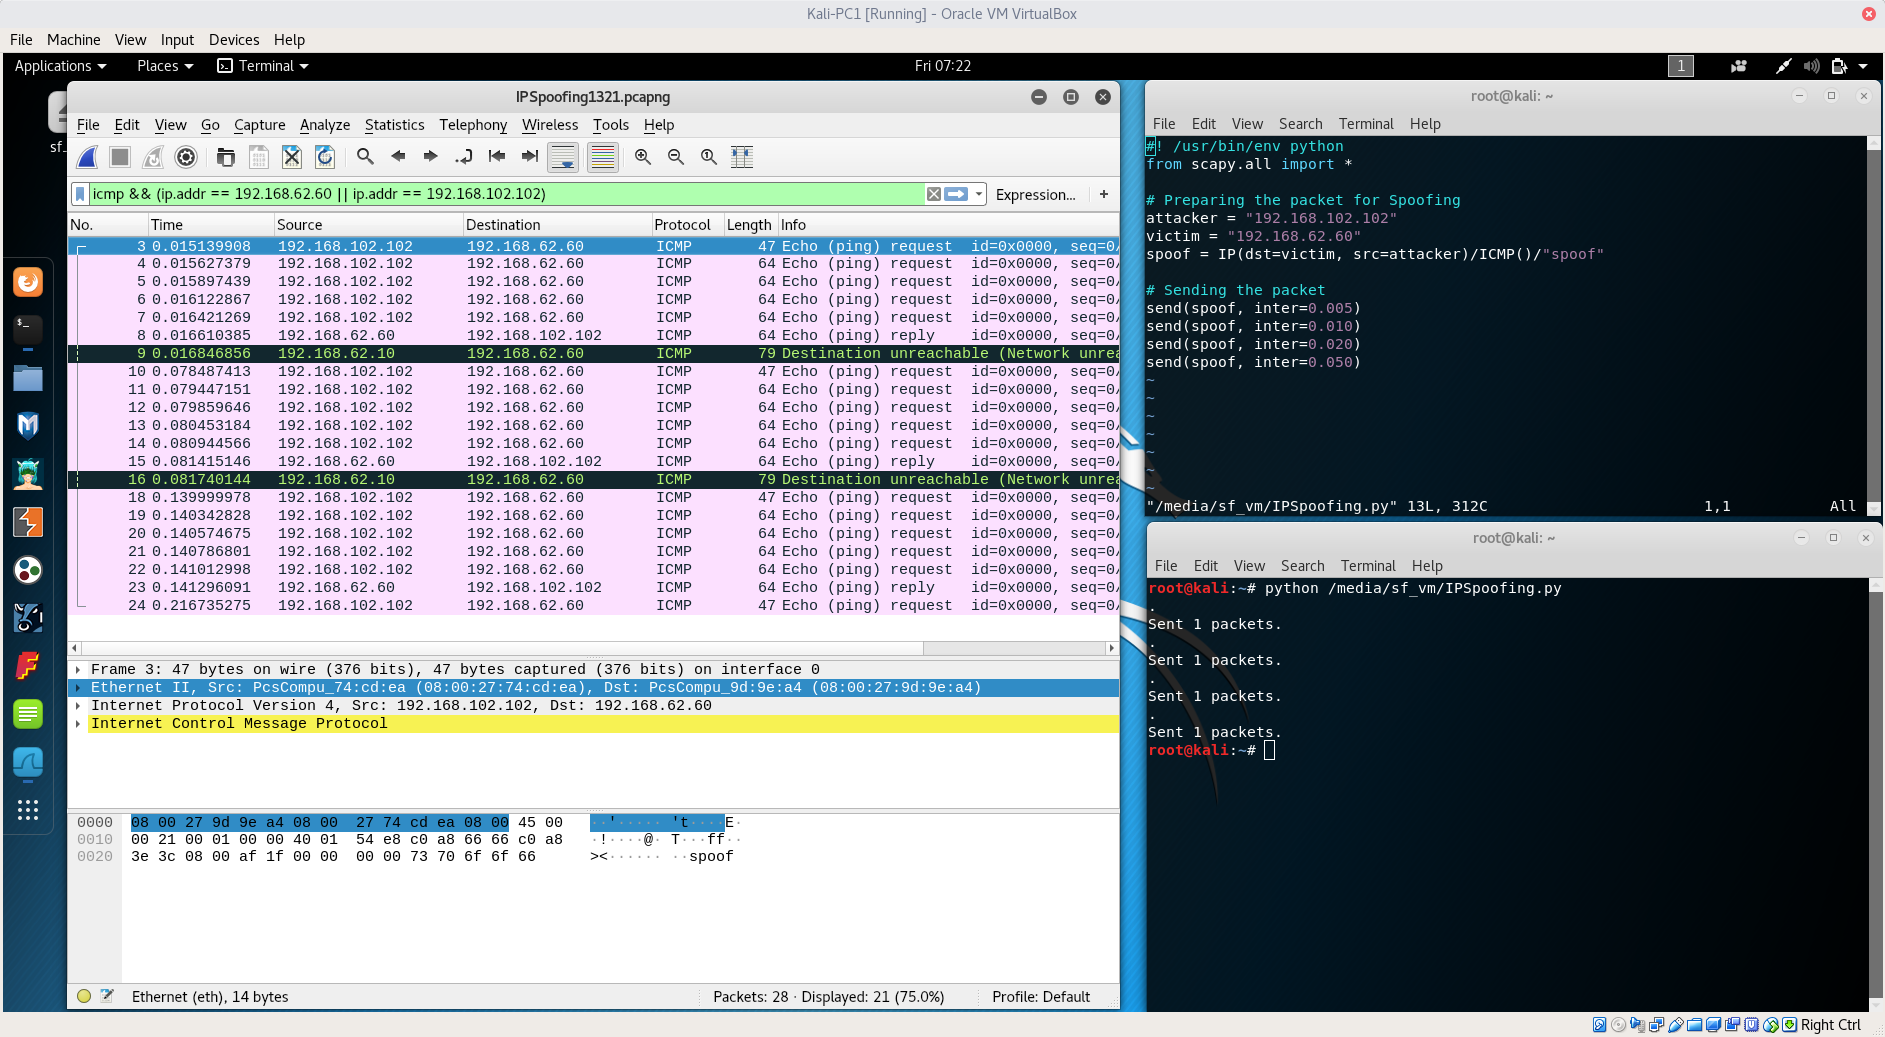
\includegraphics[width=16cm]{img/IPSpoofing.png}

% Explanation of the result of the attack
\subsubsection{Attack's result}


% Method recommended to protect the Network against such an attack
\subsubsection{How to protect the network}
